\scanpage{298}
\diagram{\begin{tikzcd}[column sep=small]
&X_1\amalg_Y X_2&\\
X_1\arrow[ur]&&X_2\arrow[ul]\\
&Y\arrow[ul,"\varphi_1"]\arrow[ur,"\varphi_2"']&
\end{tikzcd}}
\diagram{\begin{tikzcd}
X_1\amalg_Y X_2\\
X_1\amalg X_2\arrow[u]\arrow[r,dash]&{}\\
Y\arrow[u,shift left]\arrow[u,shift right]
\end{tikzcd}}
\margin{Contre-exemples par \deleted{\unsure{re}} recollement}

$\varphi_i$ immersions

\uline{exemple !}
\[
X_1=X_2=\overbrace{\operatorname{Spec}k[x,y]}^{\deleted{\unsure{X}}}-\text{origine}
\]
\[
\underbrace{\deleted{Y=\operatorname{Spec}k[t]-\text{origine}}}_{\inserted{Z}}=\operatorname{Spec}k[t,t^{-1}]
\]
$\varphi_1$ \unsure{induit} par \deleted{\unsure{$k[t]\to$}} $\deleted{Y}\inserted{Z}\to X$ défini par les équations :
\[
x=\deleted{\unsure{\varphi_1^*x}}t,\quad y=0
\]
\deleted{$\varphi_2\quad\unsure{Z}\to X\quad x=\unsure{1/t}$}

\deleted{$\varphi_2=\varphi_1\psi\quad\unsure{=}\quad\psi$}
\[
x=1/t,\quad y=0
\]
\figure{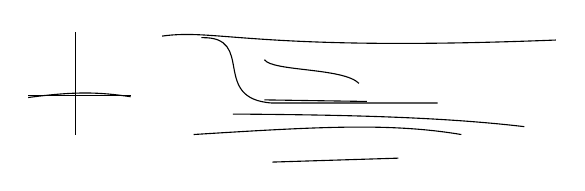
\begin{tikzpicture}[x=1cm,y=1cm]
\draw (0,0)--(1.3,0) (.6,-.5)--(.6,.8);\draw (0,-.03)..controls (.6,.05) and (.9,.04)..(1.3,-.02);
\draw (1.7,.75)..controls (2.4,.85) and (2.9,.55)..(6.7,.7);\draw (2.2,.73)..controls (2.9,.75) and (2.3,-.05)..(3.1,-.1)--(5.2,-.1);
\draw (3,.45)..controls (3.1,.3) and (4,.35)..(4.2,.15);\draw (3,-.06)--(4.3,-.08);
\draw (2.6,-.24)..controls (3.9,-.25) and (5.2,-.27)..(6.3,-.4);\draw (2.1,-.5)..controls (3.7,-.4) and (4.6,-.35)..(5.5,-.5);\draw (3.1,-.85)--(4.7,-.8);
\end{tikzpicture}}

$X'=X_1\amalg X_2$ est \unsure{quasi-affine}.

$X=X_1\amalg_Y X_2$ \unsure{ne l'est pas, car}

$\Gamma(X,\mathcal O_X)=$ \deleted{\unsure{anneau}} \unsure{sous-anneau} de $\Gamma(X')$ formé des $(f_1,f_2)$ telles que
\[
f_1\deleted{\unsure{(t,0)}}\circ\varphi_1=f_2\circ\varphi_2.
\]
Or $\Gamma(X_i,\mathcal O_{X_i})=k[x,y]$, et on a
\[
f_1(t,0)=f_2(1/t,0)
\]
\mspage{297}
